\documentclass[uplatex,dvipdfmx]{jsarticle}
\usepackage{amsmath,amssymb,amsthm}
\usepackage{mathtools}
\usepackage{mathrsfs}
% \usepackage[top=2.5cm, bottom=2.5cm]{geometry}
\usepackage[dvipdfmx]{graphicx}
\usepackage{here}
\usepackage{enumerate}
\usepackage{algorithm}
\usepackage{algpseudocode}
\usepackage{colortbl}
\usepackage{color}
\usepackage{listings}
\usepackage{tikz}
\usepackage[dvipdfmx]{hyperref}

\DeclareMathOperator*{\argmin}{arg\,min}
\DeclareMathOperator*{\argmax}{arg\,max}
\DeclareMathOperator*{\rank}{rank}
\DeclareMathOperator{\Ima}{Im}

\newcommand{\transposed}[1]{#1^\mathsf{T}}

\newtheorem*{lemma}{Lemma}
\newtheorem{definition}{Definition}

\title{最適化手法 レポート}
\author{J4-190507 2年 木下裕太}

\begin{document}
  \maketitle

  準ニュートン法はバグが取れず、再急降下法とニュートン法の2つについてシミュレーションを行いました。ソースコードは\href{https://github.com/jellc/optimization}{ここ}にあります 。\\

  \section{再急降下法}

  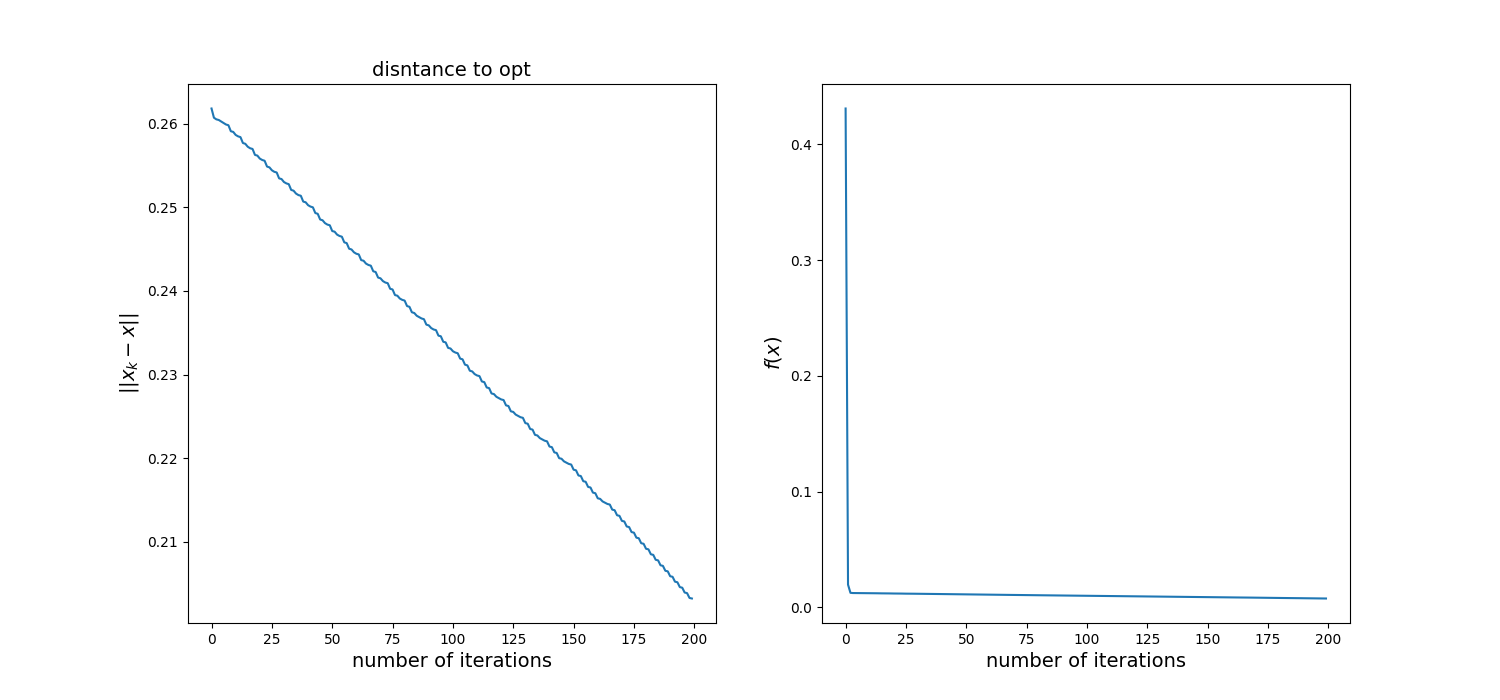
\includegraphics[scale=0.4]{out/steepest1.png}
  初期値を$(1.2, 1.2)$とした場合、上図のような挙動を示しました。\\


  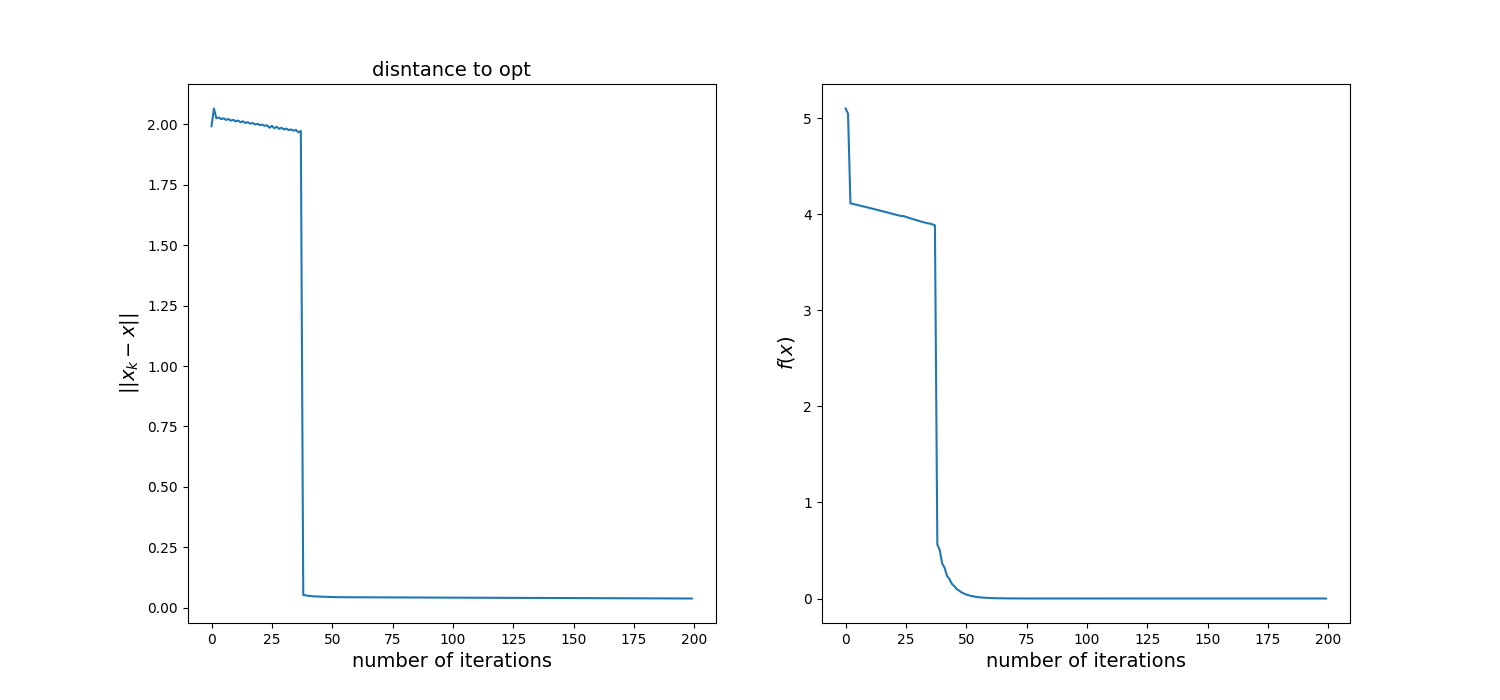
\includegraphics[scale=0.4]{out/steepest2.png}
  次に初期値を$(-1.2, 1.0)$とした場合、上図のような挙動を示しました。\\


  \section{ニュートン法}

  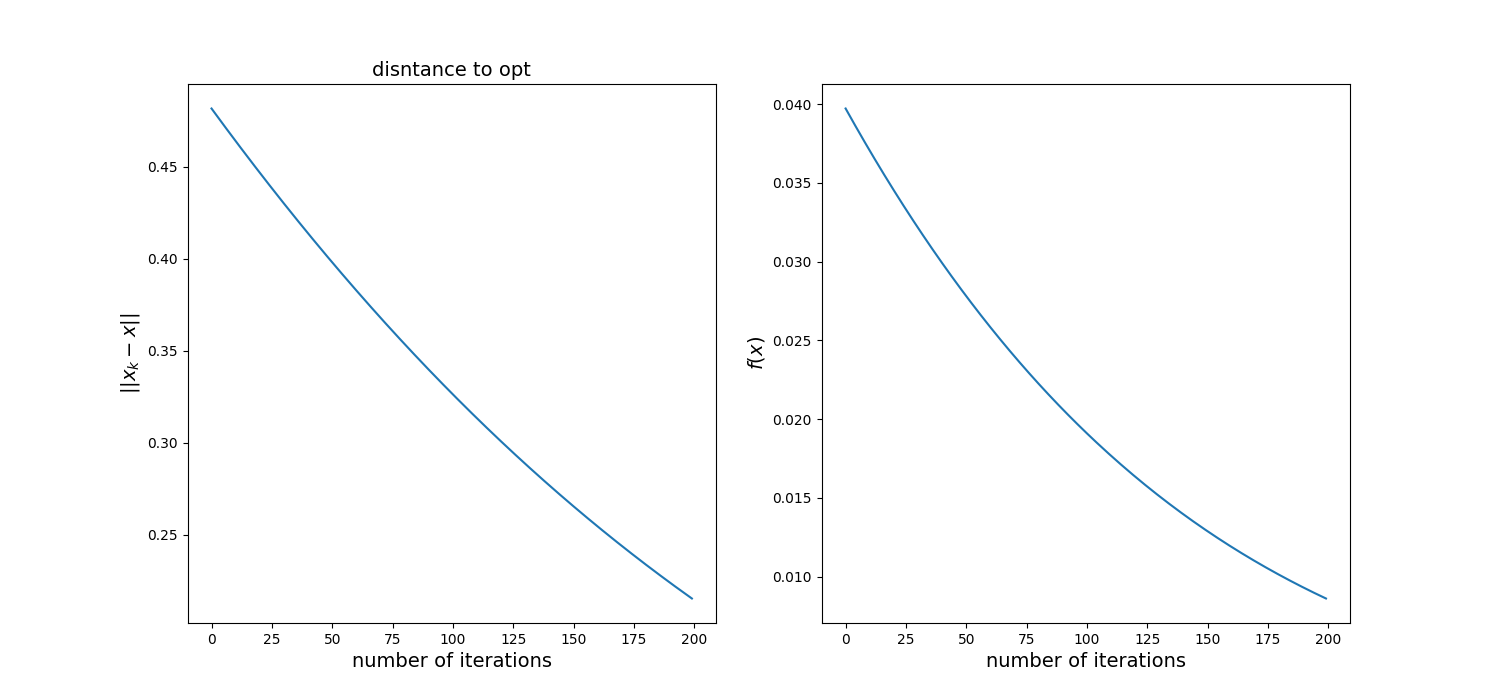
\includegraphics[scale=0.4]{out/newton1.png}
  初期値を$(1.2, 1.2)$とした場合、上図のような挙動を示しました。\\

  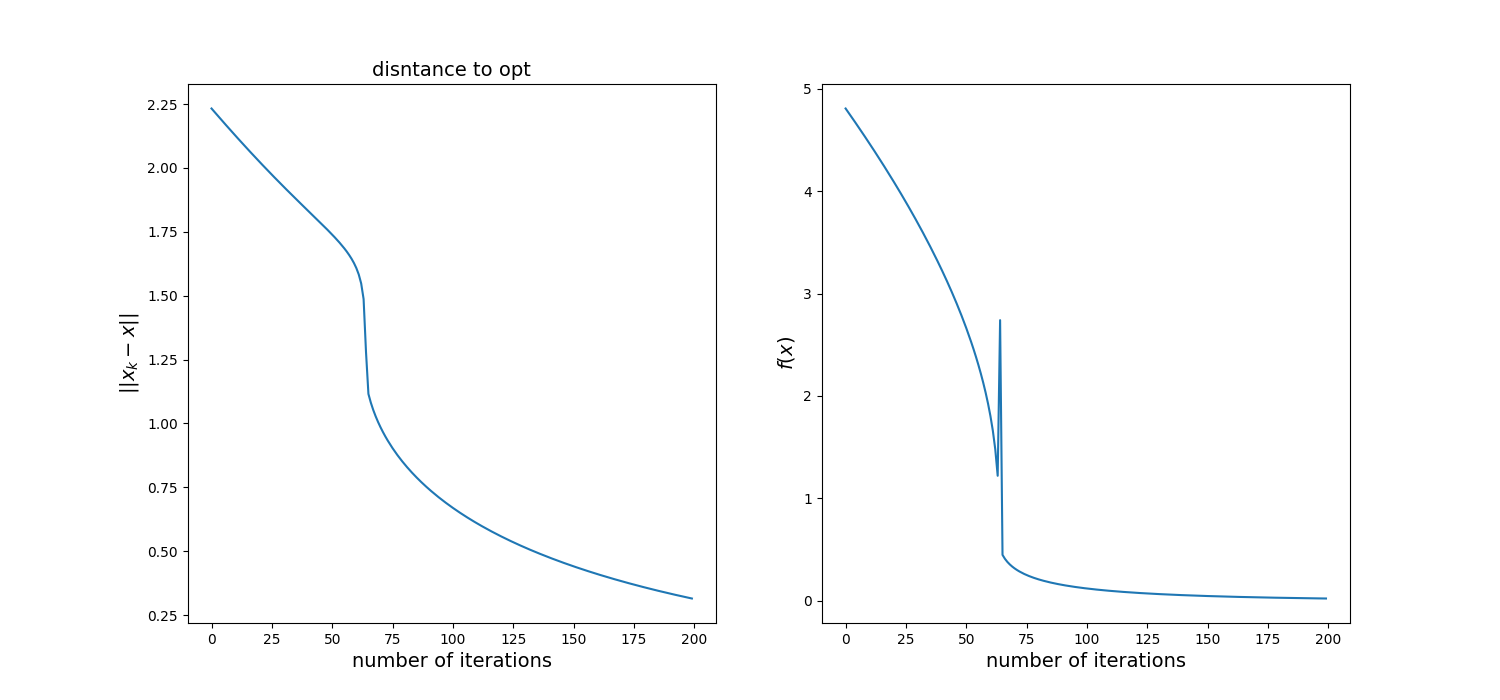
\includegraphics[scale=0.4]{out/newton2.png}
  次に初期値を$(-1.2, 1.0)$とした場合、上図のような挙動を示しました。\\
  実装が正確に行えていない可能性も考えられますが、今回の問題ではいずれの初期点からも再急降下法の方がより速く収束へ向かいました。

\end{document}
